\documentclass[12pt,a4paper]{article} % Use A4 paper with a 12pt font size - different paper sizes will require manual recalculation of page margins and border positions 

\usepackage{marginnote} % Required for margin notes
\usepackage{wallpaper} % Required to set each page to have a background
\usepackage{lastpage} % Required to print the total number of pages
\usepackage[left=1.3cm,right=2.0cm,top=1.8cm,bottom=5.0cm,marginparwidth=3.4cm]{geometry} % Adjust page margins
\usepackage{amsmath} % Required for equation customization
\usepackage{amssymb} % Required to include mathematical symbols
\usepackage{xcolor} % Required to specify colors by name
\usepackage{mdframed}
\usepackage{listings}
\definecolor{light-gray}{gray}{0.95} 
\usepackage{fancyhdr} % Required to customize headers
\usepackage[brazil]{babel}
% \usepackage[latin1]{inputenc}
%\usepackage[T1]{fontenc} 
\usepackage{graphicx}
\lstset{breaklines=true}

\usepackage{pstricks}
\usepackage{subfigure}
\usepackage{caption}  %
\captionsetup{justification=centering,labelfont=bf}
\usepackage{textcomp}
\setlength{\headheight}{80pt} % Increase the size of the header to accommodate meta-information
\pagestyle{fancy}\fancyhf{} % Use the custom header specified below
\renewcommand{\headrulewidth}{0pt} % Remove the default horizontal rule under the header

\setlength{\parindent}{0cm} % Remove paragraph indentation
\newcommand{\tab}{\hspace*{2em}} % Defines a new command for some horizontal space

\newcommand\BackgroundStructure{ % Command to specify the background of each page
\setlength{\unitlength}{1mm} % Set the unit length to millimeters

\setlength\fboxsep{0mm} % Adjusts the distance between the frameboxes and the borderlines
\setlength\fboxrule{0.5mm} % Increase the thickness of the border line
\put(10, 20pr){\fcolorbox{black}{gray!5}{\framebox(155,247){}}} % Main content box
\put(165, 20){\fcolorbox{black}{gray!10}{\framebox(37,247){}}} % Margin box
\put(10, 262){\fcolorbox{black}{white!10}{\framebox(192, 25){}}} % Header box
\put(175, 263){\includegraphics[height=23mm,keepaspectratio]{}} % Logo box - maximum height/width: 
}

%----------------------------------------------------------------------------------------
%	HEADER INFORMATION
%----------------------------------------------------------------------------------------


%----------------------------------------------------------------------------------------

\begin{document}

%\AddToShipoutPicture{\BackgroundStructure} % Set the background of each page to that specified above in the header information section

%----------------------------------------------------------------------------------------
%	DOCUMENT CONTENT
%----------------------------------------------------------------------------------------

\begin{titlepage}
   \vspace*{\stretch{1.0}}
   \begin{center}
      \Large\textbf{AppArmor - Technical report}\\
      \large\textit{Luka Minjoraia}
   \end{center}
   \vspace*{\stretch{2.0}}
\end{titlepage}


\section{Introduction}
The aim is to study is to deliver fully documented technical report about AppArmor, its features and all the other technology that was used to fulfill this project. 
\section{Definition and Methods}
\subsection{What is AppArmor?}
Apparmor is a Mandatory Access Control system which uses LSM kernel enhancements to restrict programs to certain resources. AppArmor does this with profiles loaded into the kernel when the system starts. Apparmor has two types of profile modes, enforcement and complain. Profiles in enforcement mode enforce that profile's rules and report violation attempts in syslog or auditd. Profiles in complain mode don't enforce any profile rules, their purpose is to monitor and log violation attempts.
\subsection{Methods}
The report in this paper, will go through the work that has been done, which is divided by two parts - 1)development, application and testing of custom AppArmor profiles. 2) Development of python-based application for reducing the routine operation inflexibility and attempting to develop a monitoring system, Both types of the works will be briefly discussed in the paper.



\section{Custom profiling for Securing Services and Applications using AppArmor }
AppArmor is a powerful MAC system and it has some built-in profiles for commonly used application, so I decided to make a custom profile for something that I'd perhaps use in future and it is not already in the list of built-in profiles, which is Nginx.

\subsection{Custom Profile for Nginx}
The profile primarily will restrict access to certain directories and allow certain ones, to demonstrate that I will create two directories \begin{mdframed}[backgroundcolor=light-gray, roundcorner=10pt,leftmargin=1, rightmargin=1, innerleftmargin=15, innertopmargin=15,innerbottommargin=15, outerlinewidth=1, linecolor=light-gray]
\begin{lstlisting}[language=C]
luka@luka-VirtualBox:~$ sudo mkdir -p /www/allowed
luka@luka-VirtualBox:~$ sudo mkdir -p /www/notallowed
\end{lstlisting} \end{mdframed}

Then index.html files inside these directories : 
\begin{mdframed}[backgroundcolor=light-gray, roundcorner=10pt,leftmargin=1, rightmargin=1, innerleftmargin=15, innertopmargin=15,innerbottommargin=15, outerlinewidth=1, linecolor=light-gray] \begin{lstlisting}[language=html] 
luka@luka-VirtualBox:~$ sudo nano /www/allowed/index.html
...
<html>
    <h1 Safe space </h1>
</html>
luka@luka-VirtualBox:~$ sudo nano /www/notallowed/index.html
...
<html>
    <h1 Unsafe space </h1>
</html>
\end{lstlisting} \end{mdframed}
Next, nginx configuration fine is modified and ngix service restarted. 
\begin{mdframed}[backgroundcolor=light-gray, roundcorner=10pt,leftmargin=1, rightmargin=1, innerleftmargin=15, innertopmargin=15,innerbottommargin=15, outerlinewidth=1, linecolor=light-gray] \begin{lstlisting}[language=python] 
luka@luka-VirtualBox:~$ sudo nano /etc/nginx/nginx.conf
user www-data;
worker_processes auto;
pid /run/nginx.pid;
include /etc/nginx/modules-enabled/*.conf;
events {
	worker_connections 768;
	# multi_accept on;
}
http {

	sendfile on;
	tcp_nopush on;
	tcp_nodelay on;
	keepalive_timeout 65;
	types_hash_max_size 2048;

	include /etc/nginx/mime.types;
	default_type application/octet-stream;

	ssl_protocols TLSv1 TLSv1.1 TLSv1.2; 
	ssl_prefer_server_ciphers on;

	access_log /var/log/nginx/access.log;
	error_log /var/log/nginx/error.log;

	include /etc/nginx/conf.d/*.conf;
	include /etc/nginx/sites-enabled/*;

	server {
		listen     8080;
		location   /{
                            root /www;
   }
	}
#}
}


luka@luka-VirtualBox:~$ sudo nginx -s reload

\end{lstlisting} \end{mdframed}
Now both directories are available, next step is to create a profile.
\begin{mdframed}[backgroundcolor=light-gray, roundcorner=10pt,leftmargin=1, rightmargin=1, innerleftmargin=15, innertopmargin=15,innerbottommargin=15, outerlinewidth=1, linecolor=light-gray] \begin{lstlisting}[language=C]
luka@luka-VirtualBox:/etc/apparmor.d$ sudo aa-autodep nginx
Writing updated profile for /usr/sbin/nginx
\end{lstlisting} \end{mdframed}
That will generate a AppArmor profile, now policies need to be entered to limit the access to the directory.
\begin{mdframed}[backgroundcolor=light-gray, roundcorner=10pt,leftmargin=1, rightmargin=1, innerleftmargin=15, innertopmargin=15,innerbottommargin=15, outerlinewidth=1, linecolor=light-gray] \begin{lstlisting}[language=C]
sudo gedit /etc/apparmor.d/usr.sbin.nginx
...
# Last Modified: Sun Jun 28 19:05:18 2020
#include <tunables/global>
/usr/sbin/nginx {
  #include <abstractions/apache2-common>
  #include <abstractions/base>
  #include <abstractions/nis>
  capability dac_override,
  capability dac_read_search,
  capability net_bind_service,
  capability setgid,
  capability setuid,
  /www/allowed/* r,
  deny /data/www/notallowed/* r,
  /etc/group r,
  /etc/nginx/conf.d/ r,
  /etc/nginx/mime.types r,
  /etc/nginx/nginx.conf r,
  /etc/nsswitch.conf r,
  /etc/passwd r,
  /etc/ssl/openssl.cnf r,
  /run/nginx.pid rw,
  /usr/sbin/nginx mr,
  /var/log/nginx/access.log w,
  /var/log/nginx/error.log w,
}
\end{lstlisting} \end{mdframed}
"deny /www/notallowed/* r," is the policy that completely disallows the directory, let's see by enforcing the profile and testing it.

\begin{mdframed}[backgroundcolor=light-gray, roundcorner=10pt,leftmargin=1, rightmargin=1, innerleftmargin=15, innertopmargin=15,innerbottommargin=15, outerlinewidth=1, linecolor=light-gray] \begin{lstlisting}[language=C]
 sudo aa-enforce nginx
Setting /usr/sbin/nginx to enforce mode.
 sudo /etc/init.d/apparmor reload
[ ok ] Reloading apparmor configuration (via systemctl):
 sudo service nginx restart
\end{lstlisting} \end{mdframed}

The directory /notallowed is no longer accessible.

    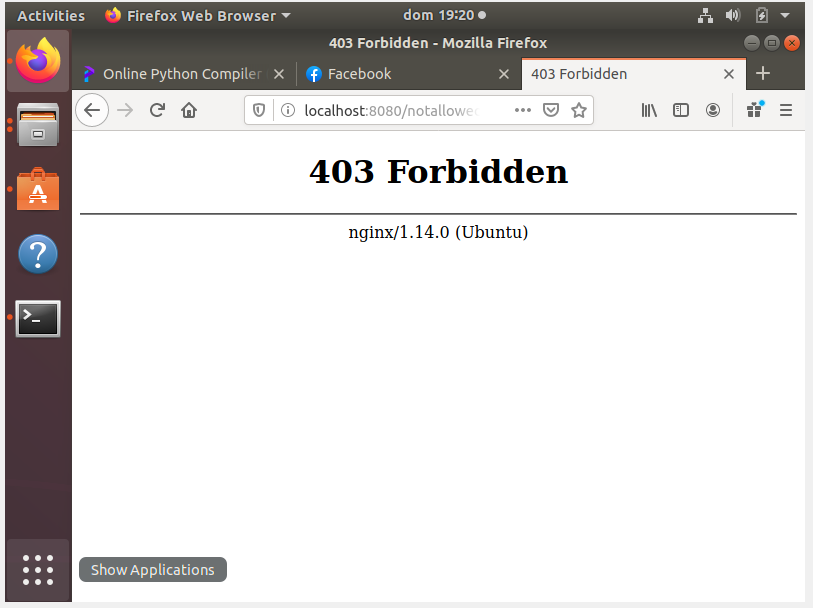
\includegraphics[width=\textwidth, height=300px]{snip1.1.PNG}


\section{Command-line based python application for AppArmor re-interpretation}

The python application is realized through embedding it into command-line based application, main objective is to ease the inflexibility of AppArmor, provide better filtered results and implement a monitoring system.

\subsection{Introduction}
The app is made through making python files executable - each command represents each executable that references main module, path is globalized in environment file.

\subsection{Source code and demonstration}

Main code is centralized in main.py which looks like this : 
\begin{mdframed}[backgroundcolor=light-gray, roundcorner=10pt,leftmargin=1, rightmargin=1, innerleftmargin=15, innertopmargin=15,innerbottommargin=15, outerlinewidth=1, linecolor=light-gray] \begin{lstlisting}[language=python]
#!/usr/bin/python3.8
import subprocess
import json
import os
import argparse
class AppArmorService:
    def get_profiles(self):
	    result = subprocess.run(['sudo','apparmor_status', '--json'], stdout=subprocess.PIPE)    
	    data = result.stdout.decode('utf-8')
	    p_status = json.loads(data)
	    return p_status
    def get_unconfined(self):
        result = subprocess.run(['sudo', 'aa-unconfined', '--paranoid'
                                ], stdout=subprocess.PIPE)
        data = result.stdout.decode('utf-8')
        lines = data.split('\n')
        apps = []
        for line in lines:
            app = line.split(' ')
            if len(app) > 1:
                apps.append((app[0], app[1]))
        return apps
    def disable_profile(self,profile):
        os.system('sudo ln -s ' + profile + ' /etc/apparmor.d/disable/')]
\end{lstlisting} \end{mdframed}

This module contains a class, containing the functionality of each command, which are executed from the separate module - let's take "aa-profiles"
\begin{mdframed}[backgroundcolor=light-gray, roundcorner=10pt,leftmargin=1, rightmargin=1, innerleftmargin=15, innertopmargin=15,innerbottommargin=15, outerlinewidth=1, linecolor=light-gray] \begin{lstlisting}[language=python]
#!/usr/bin/env python3.8
import main
service = main.AppArmorService()
profile_iterator = service.get_profiles()
print('version: ' + profile_iterator['version'])
for profile in profile_iterator['profiles']:
   status = profile_iterator["profiles"][profile]
   print(status + " " + profile)
\end{lstlisting} \end{mdframed}
Service is retrieved, formated and outputted - let's test it out, all I need to run is : "aa-profiles" to retrieve the status + profile.

    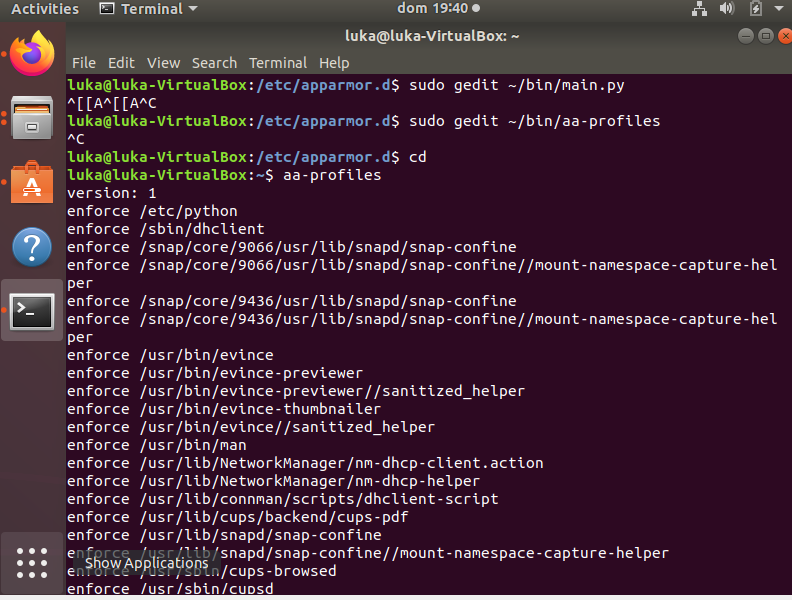
\includegraphics[width=\textwidth]{snip1.2.PNG}
\section{Conclusion}
The assignment has been incredibly productive on many levels, starting from AppArmor and Linux-python interactions, ending with understanding how internal Linux systems work during the profiling.
All of the code that has been used here is uploaded on github : https://github.com/Lukaa0/Python-AppArmor and on Virtual.IPB.
\end{document}